\section{zesto-decode.cpp File Reference}
\label{zesto-decode_8cpp}\index{zesto-decode.cpp@{zesto-decode.cpp}}
{\tt \#include \char`\"{}thread.h\char`\"{}}\par
{\tt \#include \char`\"{}zesto-core.h\char`\"{}}\par
{\tt \#include \char`\"{}zesto-opts.h\char`\"{}}\par
{\tt \#include \char`\"{}zesto-oracle.h\char`\"{}}\par
{\tt \#include \char`\"{}zesto-decode.h\char`\"{}}\par
{\tt \#include \char`\"{}zesto-fetch.h\char`\"{}}\par
{\tt \#include \char`\"{}zesto-bpred.h\char`\"{}}\par
{\tt \#include \char`\"{}zesto-cache.h\char`\"{}}\par
{\tt \#include \char`\"{}sim.h\char`\"{}}\par
{\tt \#include \char`\"{}zesto-uncore.h\char`\"{}}\par
{\tt \#include \char`\"{}zesto-MC.h\char`\"{}}\par
{\tt \#include \char`\"{}zesto-dram.h\char`\"{}}\par
{\tt \#include \char`\"{}ZPIPE-decode.list\char`\"{}}\par


Include dependency graph for zesto-decode.cpp:\nopagebreak
\begin{figure}[H]
\begin{center}
\leavevmode
\includegraphics[width=420pt]{zesto-decode_8cpp__incl}
\end{center}
\end{figure}
\subsection*{Functions}
\begin{CompactItemize}
\item 
void {\bf decode\_\-reg\_\-options} (struct {\bf opt\_\-odb\_\-t} $\ast$odb, struct {\bf core\_\-knobs\_\-t} $\ast${\bf knobs})
\item 
class {\bf core\_\-decode\_\-t} $\ast$ {\bf decode\_\-create} (const char $\ast$decode\_\-opt\_\-string, struct {\bf core\_\-t} $\ast$core)
\end{CompactItemize}


\subsection{Function Documentation}
\index{zesto-decode.cpp@{zesto-decode.cpp}!decode\_\-create@{decode\_\-create}}
\index{decode\_\-create@{decode\_\-create}!zesto-decode.cpp@{zesto-decode.cpp}}
\subsubsection[{decode\_\-create}]{\setlength{\rightskip}{0pt plus 5cm}class {\bf core\_\-decode\_\-t}$\ast$ decode\_\-create (const char $\ast$ {\em decode\_\-opt\_\-string}, \/  struct {\bf core\_\-t} $\ast$ {\em core})}\label{zesto-decode_8cpp_4fc719f96861588f24dd802be6e2b0df}




Definition at line 144 of file zesto-decode.cpp.

References fatal().

Referenced by sim\_\-post\_\-init().

Here is the caller graph for this function:\nopagebreak
\begin{figure}[H]
\begin{center}
\leavevmode
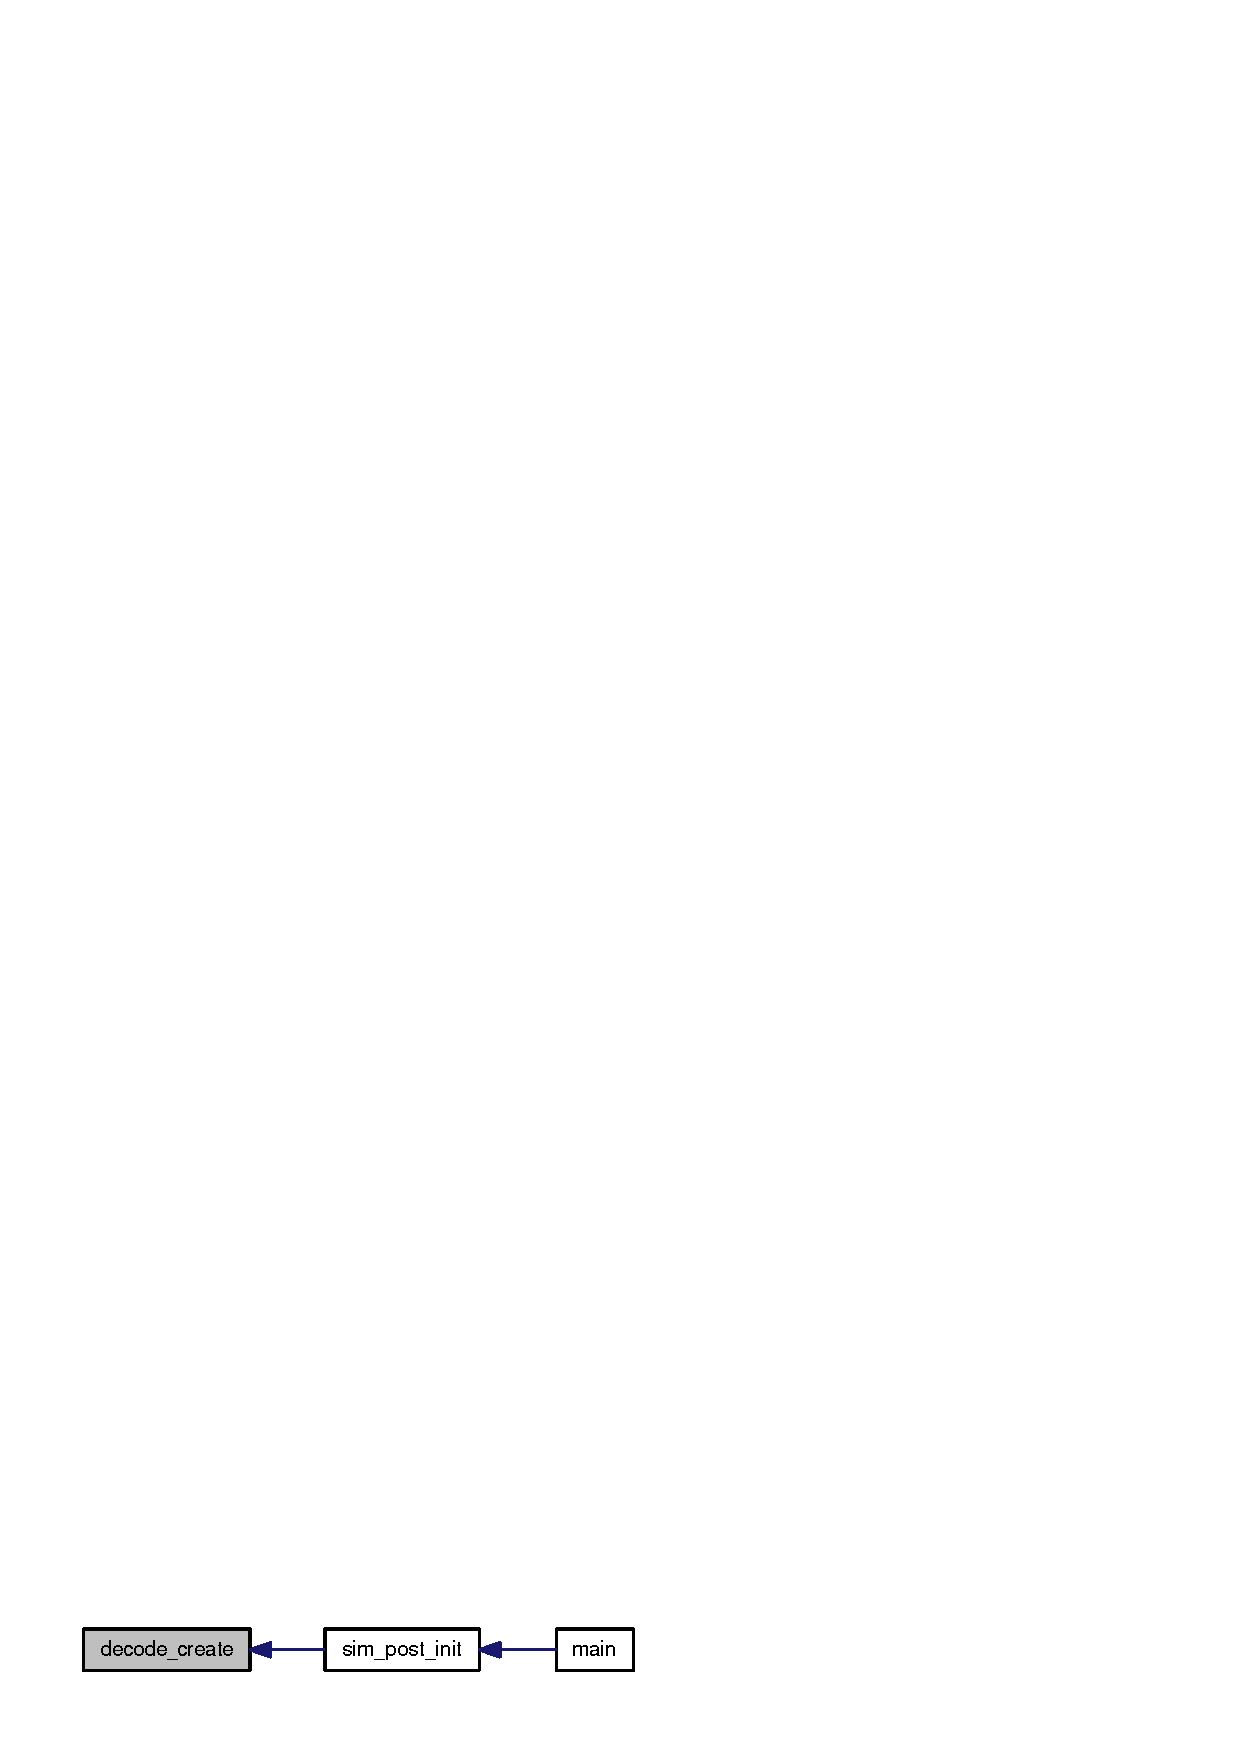
\includegraphics[width=154pt]{zesto-decode_8cpp_4fc719f96861588f24dd802be6e2b0df_icgraph}
\end{center}
\end{figure}
\index{zesto-decode.cpp@{zesto-decode.cpp}!decode\_\-reg\_\-options@{decode\_\-reg\_\-options}}
\index{decode\_\-reg\_\-options@{decode\_\-reg\_\-options}!zesto-decode.cpp@{zesto-decode.cpp}}
\subsubsection[{decode\_\-reg\_\-options}]{\setlength{\rightskip}{0pt plus 5cm}void decode\_\-reg\_\-options (struct {\bf opt\_\-odb\_\-t} $\ast$ {\em odb}, \/  struct {\bf core\_\-knobs\_\-t} $\ast$ {\em knobs})}\label{zesto-decode_8cpp_22a8e8da3f62458e0ed1dd350cec4ae7}




Definition at line 89 of file zesto-decode.cpp.

References core\_\-knobs\_\-t::branch\_\-decode\_\-limit, core\_\-knobs\_\-t::decode, core\_\-knobs\_\-t::decoders, core\_\-knobs\_\-t::depth, core\_\-knobs\_\-t::fusion\_\-all, core\_\-knobs\_\-t::fusion\_\-load\_\-op, core\_\-knobs\_\-t::fusion\_\-none, core\_\-knobs\_\-t::fusion\_\-partial, core\_\-knobs\_\-t::fusion\_\-sta\_\-std, MAX\_\-DECODE\_\-WIDTH, core\_\-knobs\_\-t::MS\_\-latency, core\_\-knobs\_\-t::num\_\-decoder\_\-specs, opt\_\-reg\_\-flag(), opt\_\-reg\_\-int(), opt\_\-reg\_\-int\_\-list(), core\_\-knobs\_\-t::target\_\-stage, core\_\-knobs\_\-t::uopQ\_\-size, and core\_\-knobs\_\-t::width.